\chapter{Neutrino Physics}\label{chapter:NeutrinoPhysics}

\section{History}
The neutrino was first proposed by Wolfgang Pauli in December 1930 as a radical solution to the problem of energy conservation in beta decay. It had been observed that the electron from beta decay had a continuous energy distribution, which could only be consistent with the law of conservation of energy if a third particle was also emitted. This particle, which Pauli called a \emph{neutron}, was incorporated into Enrico Fermi's 1934 theory of beta decay as the \emph{neutrino}~\citep{Fermi1934,Wilson1968}. The neutrino was postulated to be (almost) massless and electrically neutral. Its role in beta decay meant it must carry spin $\half$. The neutrino remained a theoretical ghost until it was conclusively discovered in 1956 by Frederick Reines and Clyde Cowan~\citep{Reines1956}, in an experiment which agreed with the predicted interaction cross-section of $6.3\times 10^{-44} \cm^2$.

In 1964, John Bahcall published a solar model which predicted the neutrino flux from the Sun~\citep{Bahcall1964}. This model was put to the test by Raymond Davis, Jr. in what is now known as the Homestake experiment~\citep{Davis1964}; a carefully designed radiochemical experiment which measured the solar neutrino flux by counting the decays of $^{37}\Ar$ atoms which were produced in charged current neutrino interactions on $^{37}\Cl$ nuclei. After a period of 20 years of data-taking, theoretical and experimental refinements, the Homestake experiment concluded that there was a discrepancy between experiment and theory; the rate measured experimentally was approximately one third the predicted rate. This became known as the \emph{solar neutrino problem}.

Meanwhile, it was discovered that the neutrino that appears in pion decay ($\pi^\pm \rightarrow \mu^\pm + \nu$) differs somehow from that produced in $\beta$ decay~\citep{Danby1962}; the neutrinos from pion decay always produced muons in a charged current interaction, while those from $\beta$ decay produced electrons. This distinction between neutrino \emph{flavours} led Pontecorvo to predict mixing (\emph{oscillation}) between neutrino flavours in 1958~\citep{Pontecorvo1958}, and in particular $\nu_e \leftrightarrow \nu_\mu$ oscillations in 1968~\citep{Pontecorvo1968}.

The Kamiokande experiment further reinforced the solar neutrino problem, with an experimental result showing that only about half of the expected neutrino flux was observed with a detection mechanism that involved imaging the Čerenkov light produced when electrons from neutrino interactions pass through water~\citep{Hirata1989}. The Kamiokande experiment was originally designed to search for proton decay, and in studying their backgrounds they discovered another problem with neutrinos; the \emph{atmospheric neutrino problem}, in which the measured flux of neutrinos from cosmic ray interactions in the atmosphere ($p\rightarrow \pi \rightarrow \mu + \nu \rightarrow \nu + e$) was only about 60\% of that expected.

With an observed deficit in both electron ($\nu_e$) and muon ($\nu_\mu$) neutrinos, the oscillation predicted by Pontecorvo provided a likely explanation, but it was only in 2002 that this was confirmed. The Sudbury Neutrino Observatory (SNO) measured the flux of $^8\mathrm{B}$ solar neutrinos~\citep{Ahmad2001} with a water Čerenkov detector filled with heavy water ($\mathrm{D}_2\mathrm{O}$). SNO was sensitive to charged current (CC), elastic scattering (ES) and neutral current (NC) neutrino interactions of the form:
\begin{eqnarray*}
CC: & \nu_e + d \rightarrow e^{-} + p + p \\
ES: & \nu + e^{-} \rightarrow \nu + e^{-} \\
NC: & \nu + d \rightarrow \nu + p + n 
\end{eqnarray*}

The Kamiokande experiment was sensitive to the CC and ES interactions, but not to the NC interaction. It was this additional sensitivity that allowed SNO to measure not only the $\nu_e$ flux, but also the \emph{total} neutrino flux, independent of flavour. While the CC flux was found to be low, by an amount consistent with Kamiokande and Homestake, the total rate of interactions from all flavours of neutrino, measured through the NC channel, implied a neutrino flux which was precisely that predicted by the solar model, and John Bahcall's work was finally validated, over 30 years after the solar neutrino problem was discovered.

The SNO results provided a clear indication that neutrino flavour oscillations were taking place: the pure $\nu_e$ from the Sun were undergoing flavour change, appearing at Earth as $\nu_\mu$ and $\nu_\tau$. The theory of neutrino oscillations---expanded by Maki, Nakagawa and Sakata in 1962~\citep{Maki1962}---requires that the neutrinos have mass, and introduces a $3\times 3$ unitary mixing matrix (the PMNS matrix) analogous to the CKM matrix\footnote{After Cabibbo, Kobayashi and Maskawa.} for quark flavour mixing (see chapter \ref{sec:neutrino_oscillations}).

It is now known that the dominant mechanism for the reduction of $\nu_e$ in the solar neutrino flux is a resonant interaction known as the MSW\footnote{After Mikheyev, Smirnov and Wolfenstein.} effect, which occurs in the electron-rich solar environment. Once the neutrinos leave the Sun, their propagation through the vacuum to Earth makes no substantial change. The MSW effect is due to charged current elastic forward scattering of neutrinos in environments where there is a high density of the corresponding flavoured charged lepton~\citep{Zuber2004}.

\section{\texorpdfstring{$\Charge\Parity$}{CP} Violation}
It is thought that in the very early universe, immediately after the big bang, matter and antimatter were created in equal amounts. The visible universe today is dominated by matter, a situation that requires some asymmetry in the way matter and antimatter interact~\citep{Perkins2000}.

This asymmetry is known as $\Charge\Parity$ violation, where $\Charge\Parity$ is the combined operation of the charge conjugation operator $\Charge$ (which swaps particles for antiparticles, and vice versa), and the parity operator $\Parity$ (which flips the signs of all spatial coordinates). $\Charge\Parity$ violation is one of the three Sakharov conditions~\citep{Sakharov1967} required to generate the measured baryon asymmetry of the universe:
\begin{enumerate}
    \item Existence of a baryon number violating process.
    \item Existence of $\Charge$ and $\Charge\Parity$ violation.
    \item Interactions outside of thermal equilibrium.
\end{enumerate}

The first condition is required in order for baryons to be produced at all. Under the assumption that such a mechanism exists, the second condition introduces an asymmetry which favours the production of baryons over that of antibaryons. This must occur outside of thermal equilibrium, such that the creation processes and annihilation processes have different rates.

$\Charge\Parity$ violation has been observed in the quark sector~\citep{PDG2012}, but the level to which it has been observed is insufficient to produce the asymmetry we see in the universe today. Neutrino oscillations open up the possibility for $\Charge\Parity$ violation to occur in the lepton sector, producing a lepton asymmetry which may then be converted to a baryon asymmetry~\citep{Riotto1999}.

\section{Neutrino Oscillations}\label{sec:neutrino_oscillations}
The mixing of three massive neutrinos can be parametrised with a $3\times 3$ unitary\footnote{$U^\dagger U = \mathbb{1}$} matrix $U$, known as the PMNS matrix.\footnote{After Pontecorvo, Maki, Nakagawa and Sakata.} The matrix $U$ relates the three neutrino flavour states $\nu_\alpha$ to the three mass states $\nu_i$. The flavour state $\rstate{\alpha}$ can be expressed as a superposition of mass states $\rstate{i}$ through components of $U$~\citep{Kayser1981}:
\begin{equation}\label{eqn:flavour_mass_mixing}
\rstate{\alpha} = \sum_i U_{\alpha i}^* \rstate{i}
\end{equation}

Given this relationship between a flavour state $\rstate{\alpha}$ and the mass states $\rstate{i}$, it is possible to determine the probability that a neutrino produced in state $\rstate{\alpha}$ is observed at some later time to be in state $\rstate{\beta}$. A full treatment is too long to describe here\footnote{See, for instance, \citep{Kayser1981} for a complete treatment using wave-packets.} so, as is traditional, several simplifications will be made. The first is to assume a plane-wave form for the neutrino states; while this is unphysical, it allows for the trivial development of the expression for the oscillation probability. It is then necessary to manually impose the requirement that the neutrino is localised in space and propagates at a fixed speed, so that the system evolves purely as a function of the distance travelled by the neutrino, $x$. Then:
\begin{equation}\label{eqn:plane_wave_nu_propagation}
\ket{\nu(x,t)} = e^{-i p\cdot x}\ket{\nu(0)} 
\end{equation}

The expression $p\cdot x = Et - \vec{p}\cdot\vec{x}$ is dependent on the mass of the neutrino involved, so it must be expanded in the mass basis as follows:
\begin{equation}\label{eqn:mass_expansion_of_propagation}
\ket{\nu(x)} = \sum_i A_i e^{-i p_i\cdot x}  \rstate{i}
\end{equation}

The amplitude $A_i$ is the amplitude of the mass state $\rstate{i}$ at $x=0$. Neutrinos are always produced as flavour eigenstates, so the amplitudes of the mass states are given by transforming using the PMNS matrix $U$:
\begin{equation}\label{eqn:mass_state_amplitudes}
A_i = \braket{\nu_i}{\nu_\alpha} = U_{\alpha i}^*
\end{equation}

After the neutrino has propagated some distance $x$ (during which time we deal with the mass states), it is detected by observing the flavour state. This requires a second transformation:
\begin{equation}\label{eqn:nu_mass_to_flavour_transf}
\lstate{\beta} = \sum_j U_{\beta j} \lstate{j}
\end{equation}

The oscillation amplitude is obtained by putting together the two transformations, along with the propagation term:\footnote{Note that $\braket{\nu_j}{\nu_i} = \delta_{ij}$, i.e. the mass states are orthogonal and are eigenstates of the Hamiltonian.}
\begin{align}\label{eqn:oscillation_amplitude}
\braket{\nu_\beta(x)}{\nu_\alpha(0)} & = \sum_j \sum_i U_{\beta j} \lstate{j} U_{\alpha i}^* e^{-i p_i\cdot x}\rstate{i} \\
 & = \sum_i U_{\beta i} U_{\alpha i}^* e^{-i p_i\cdot x} \nonumber
\end{align}

The phase $\phi_i = p_i\cdot x$ is problematic, since a plane wave has well-defined momentum and energy, and therefore mass through $E^2 = p^2 + m^2$, but we measure flavour states, not mass states\footnote{Actually, knowledge of the mass states involved destroys the oscillation probability, see \citep{Kayser1981} for details.} so we must introduce some uncertainty into the energy or the momentum. In principle, we must integrate over the range of allowed momenta, but in the spirit of simplification, a widely adopted strategy is to force all neutrino mass states to have the same momentum $\vec{p}$. This introduces small variations in energy (through the mass differences) and saves the oscillation probability. The phase is now given by:
\begin{equation}\label{eqn:phase}
\phi_i = E_i t - \vec{p}\cdot\vec{x}
\end{equation}

Under the assumption that the neutrino is highly relativistic, i.e. the mass states $m_i \ll E$, it is possible to expand:
\begin{align}\label{eqn:energy_expansion}
E_i & = \sqrt{|\vec{p}|^2 + m_i^2} \nonumber \\
 & \approx |\vec{p}|\left(1 + \frac{m_i^2}{2|\vec{p}|^2}\right) 
\end{align}

In a highly relativistic scenario, the distance $L$ from source to detector is approximately the travel time $t$, and the energy $E$ is approximately the magnitude of the momentum, $|\vec{p}|$. Making these substitutions yields:
\begin{align}\label{eqn:phase_expanded}
\phi_i &=\displaystyle |\vec{p}|\left(1 + \frac{m_i^2}{2|\vec{p}|^2}\right)L - |\vec{p}|L \\
 &= \displaystyle \frac{m_i^2 L}{2E} \nonumber
\end{align}

The oscillation probability amplitude can then be written as:
\begin{equation}\label{eqn:osc_prob_amplitude}
\braket{\nu_\beta(L)}{\nu_\alpha(0)} = \sum_i U_{\beta i} U_{\alpha i}^* \exp\left(-i \frac{m_i^2 L}{2E}\right)
\end{equation}
with a corresponding probability:\footnote{The ``distance'' labels $(L)$ and $(0)$ are omitted from this point forward.}
\begin{align}\label{eqn:osc_probability}
P(\nu_\alpha \rightarrow \nu_\beta) & = \left|\braket{\nu_\beta}{\nu_\alpha}\right|^2 \\
 & = \sum_{ij} U_{\beta i} U_{\alpha i}^* U_{\beta j}^* U_{\alpha j} \exp\left(-i\frac{(m_i^2 - m_j^2)L}{2E}\right) \nonumber
\end{align}
Writing $\Delta m_{ij}^2 = m_i^2 - m_j^2$ gives:\footnote{The rearrangement here is for convenience; the expression remains the same, but now we have two clearly identifiable terms.}
\begin{align}
P(\nu_\alpha \rightarrow \nu_\beta) = & \sum_i U_{\beta i} U_{\alpha i}^* \sum_j U_{\beta j}^* U_{\alpha j} \nonumber \\
 & + \sum_{ij} U_{\beta i} U_{\alpha i}^* U_{\beta j}^* U_{\alpha j} \left[ \exp\left(-i\frac{\Delta m_{ij}^2 L}{2E}\right) - 1\right]
 \end{align}

The first term in equation \eqref{eqn:osc_probability} reduces to $\delta_{\alpha\beta}$ since $U$ is unitary. The second term can be rewritten with the understanding that terms with $j > i$ are the complex conjugate of terms with $j < i$, and that the phase difference is $0$ when $j = i$. We now obtain:
\begin{align}\label{eqn:osc_probability_again}
P(\nu_\alpha \rightarrow \nu_\beta) = &~ \delta_{\alpha\beta} + 2\sum_{i > j} U_{\beta i} U_{\alpha i}^* U_{\beta i}^* U_{\alpha i}\left(e^{-i\Delta m_{ij}^2 L / 2E} - 1 \right) 
\end{align}

The term inside parentheses can be split into real and imaginary parts, giving (after a little effort):
\begin{align}\label{eqn:osc_prob_threeparts}
P(\nu_\alpha \rightarrow \nu_\beta) = & ~\delta_{\alpha\beta} \nonumber \\
 &~ - 4\sum_{i> j} \Re \left( U_{\beta i} U_{\alpha i}^* U_{\beta j}^* U_{\alpha j} \right) \sin^2\left(\frac{\Delta m_{ij}^2 L}{4E}\right) \nonumber \\
 &~ + 2\sum_{i> j} \phantom{^2} \Im \left( U_{\beta i} U_{\alpha i}^* U_{\beta j}^* U_{\alpha j}\right) \sin \left(\frac{\Delta m_{ij}^2 L}{2E}\right) 
\end{align}

The first term of equation \eqref{eqn:osc_prob_threeparts} states that in the absence of oscillations, we would detect the same flavour that we started with. The second term (which takes the real parts of the PMNS matrix elements, and involves a $\sin^2$ term) is $\Charge\Parity$ even, behaving identically for particles and antiparticles (for which the oscillation probability is found by taking the complex conjugate of each $U$ term). This $\Charge\Parity$ even term is responsible for neutrino oscillations. The third term is $\Charge\Parity$ odd, and disappears completely if $U$ is real.\footnote{In the special case of two neutrino flavours, $U$ must be real. This restriction is lifted for three flavours.} The third term also vanishes if we are considering \emph{survival}, i.e. $P(\nu_\alpha \rightarrow \nu_\alpha)$, for which the \emph{survival probability} is:
\begin{equation}\label{eqn:survival_probability}
P(\nu_\alpha \rightarrow \nu_\alpha) = 1 - 4\sum_{i>j} |U_{\alpha i}|^2 |U_{\alpha j}|^2 \sin^2 \left(\frac{\Delta m_{ij}^2 L}{4E}\right)
\end{equation}

\section{The PMNS Matrix}
The PMNS matrix $U$ can be parametrised by three Euler angles and (in general) six phases. For the case of three massive Dirac neutrinos ($\nu_i \ne \bar{\nu}_i$), five of the phases can be absorbed by the particle fields. Three absorbed phases correspond to unobservable rotations of the neutrino flavour eigenstates, two correspond to relative phases of the mass eigenstates. This leaves just one $\Charge\Parity$ violating Dirac phase. For Majorana neutrinos ($\nu_i = \bar{\nu}_i$) there are two additional Majorana phases, which cannot be absorbed.\footnote{Majorana neutrinos, neutrino mass mechanisms, and lepton-number violating processes such as neutrinoless double-$\beta$ decay will not be described further in this thesis. For more details, consult a good book on neutrino physics~\citep{Zuber2004,Giunti2007}.} In the usual formulation~\citep{PDG2011}, the matrix $U \equiv VP$ (where $P$ encapsulates the Majorana phases) is expressed as follows, where $c_{ij} \equiv \cos\theta_{ij}$ and $s_{ij} \equiv \sin\theta_{ij}$ represent the cosines and sines of the mixing angles.
% Can use: \enlargethispage{\baselineskip}
% to keep from splitting footnotes across the page

\begin{equation}\label{eqn:pmns-matrix_split}
V \equiv \left( \begin{array}{ccc} 1& 0 & 0 \\ 0 & c_{23} & s_{23} \\ 0 & -s_{23} & c_{23} \end{array}\right)
\left( \begin{array}{ccc} c_{13} & 0 & s_{13}e^{-i\delta} \\ 0 & 1 & 0 \\ -s_{13}e^{i\delta} & 0 & c_{13} \end{array} \right)
\left( \begin{array}{ccc} c_{12} & s_{12} & 0 \\ -s_{12} & c_{12} & 0 \\ 0 & 0 & 1 \end{array} \right)
\end{equation}

\begin{equation}\label{eqn:majorana-matrix}
P \equiv \diag \left( 1, ~ \exp\left[\frac{i\alpha_{21}}{2}\right], ~ \exp\left[\frac{i\alpha_{31}}{2}\right] \right)
\end{equation}

In the expression for $V$ above, each sub-matrix represents a rotation corresponding (roughly) to mixing between two neutrinos. This was used historically as a simplification for oscillation probability calculations, and each sub-matrix was assigned a name based on the neutrino source for an experiment which most readily provided sensitivity: ``solar'' for $\theta_{12}$, ``atmospheric'' for $\theta_{23}$, and ``reactor'' for $\theta_{13}$. The latest oscillation results are analysed in the context of a full three-neutrino mixing scenario, where it is more convenient to represent the matrix $V$ in a combined form:

\begin{equation}\label{eqn:pmns_matrix_combined}
V \equiv \left( \begin{array}{ccc}
 c_{12}c_{13} & s_{12}c_{13} & s_{13}e^{-i\delta} \\
 -s_{12}c_{23} - c_{12}s_{23}s_{13}e^{i\delta} & c_{13}c_{23} - s_{12}s_{23}s_{13}e^{i\delta} & s_{23}c_{13} \\
 s_{12}s_{23} - c_{12}c_{23}s_{13}e^{i\delta} & -c_{12}s_{23} - s_{12}c_{23}s_{13}e^{i\delta} & c_{23}c_{13}
 \end{array}
\right)
\end{equation}

\subsection{Solar Neutrinos and \texorpdfstring{$\theta_{12}$}{θ₁₂}}
The best measurements of the angle $\theta_{12}$ and the mass splitting $\Delta m^2_{21}$ come from solar neutrino experiments including the Homestake ($\Cl$), SAGE~\citep{SAGE2002}, GALLEX~\citep{GALLEX1999} and GNO~\citep{GNO2005} (all $\Ga$) radiochemical experiments, as well as from the Super-Kamiokande and SNO ($\Hydrogen_2\Oxygen$ and $\Deuterium_2\Oxygen$, respectively) water Čerenkov detectors.

From a global three-flavour oscillation analysis, taking into account data from all contributing experiments, the values for the ``solar'' parameters $\theta_{12}$ and $\Delta m^2_{21}$ are shown in figure \ref{fig:theta_12_confidence}, with contours highlighting the allowed region of the parameter space. The best-fit values are~\citep{Mezzetto2010}:
\begin{equation}\label{eqn:solar_parameters}
\sin^2 \theta_{12} = 0.318^{+0.019}_{-0.016} , ~~~~ \Delta m^2_{21} =  7.59^{+0.23}_{-0.18} \times 10^{-5} \eV^2
\end{equation}

\begin{figure}
\centering
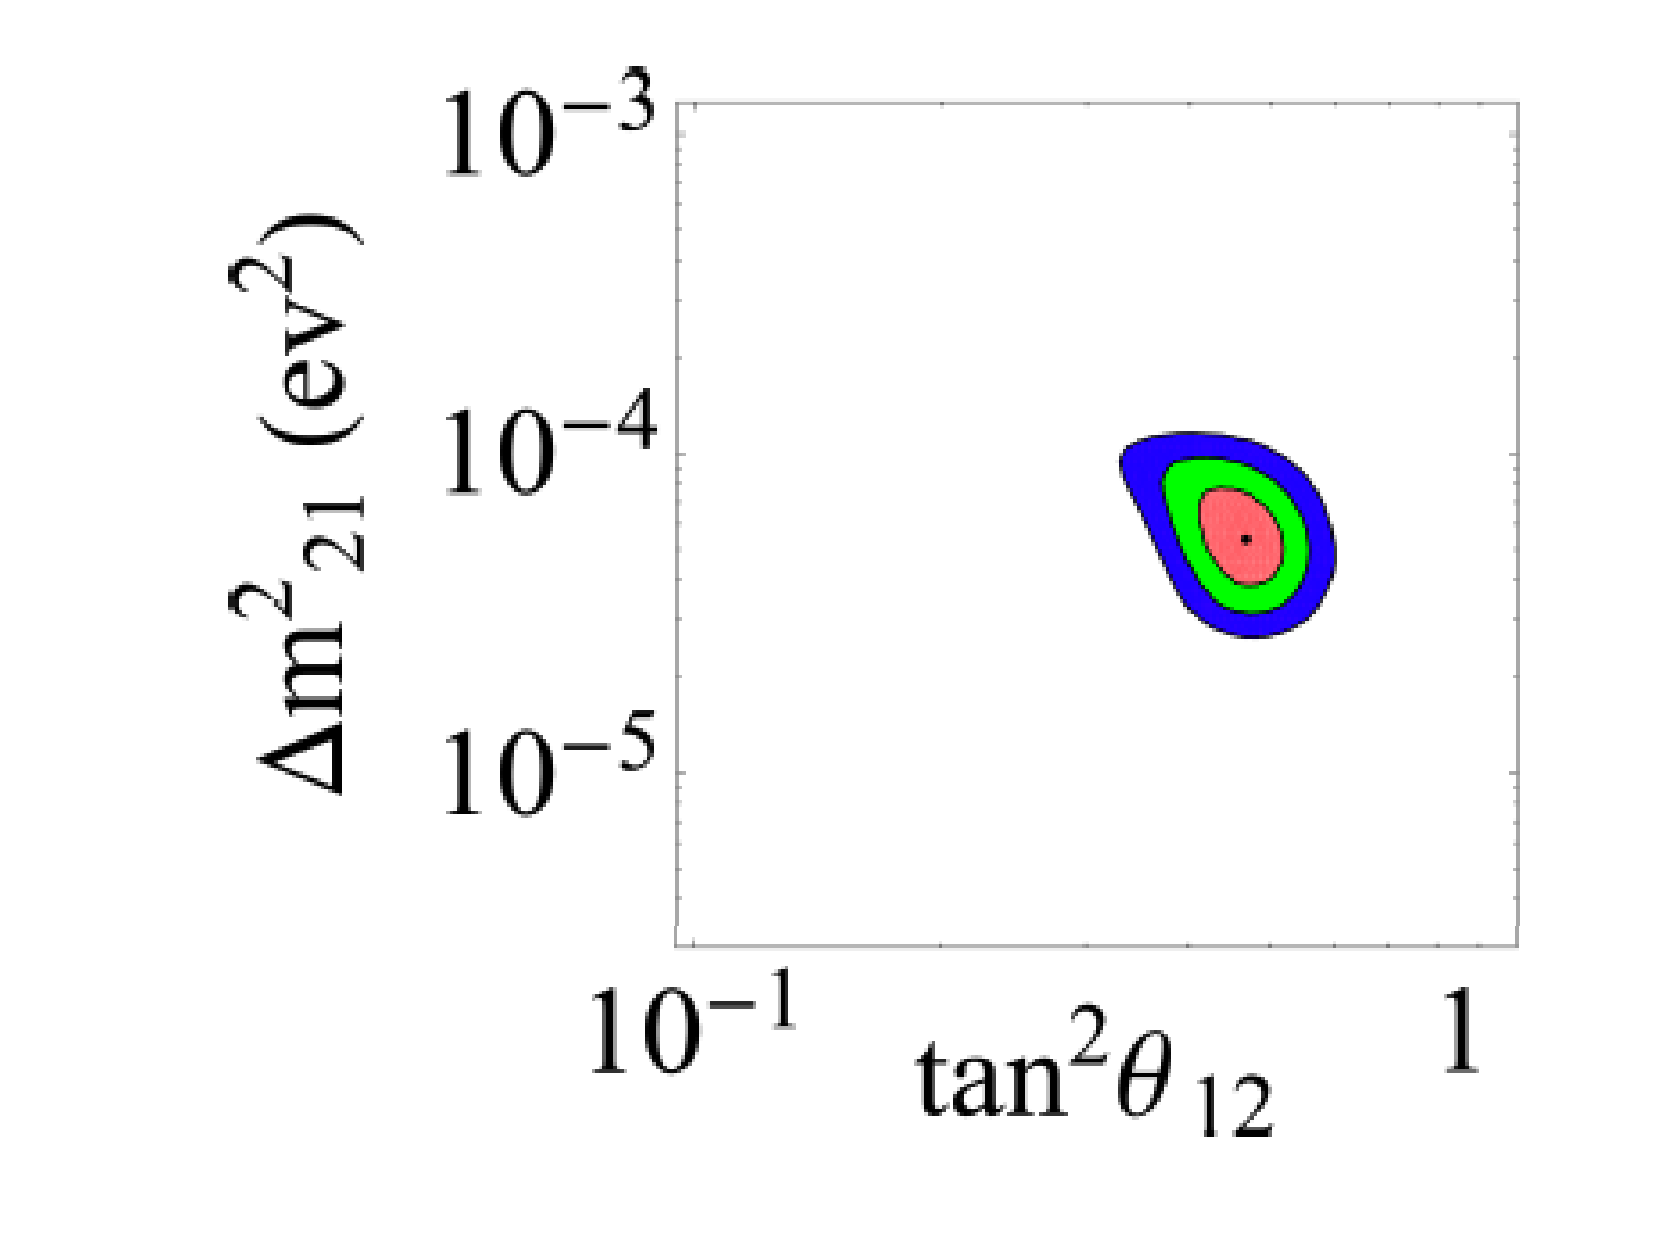
\includegraphics[width=0.6\textwidth]{chapters/neutrinophysics_images/theta_12}
\caption[Allowed region for $\theta_{12}$ and $\Delta m^2_{21}$]{\label{fig:theta_12_confidence}The current knowledge of the values of $\theta_{12}$ and $\Delta m^2_{21}$ represented as a plot of $\Delta m^2_{21}$ against $\tan^2\theta_{12}$. The contours give the $68.27\%$, $95.45\%$ and $99.74\%$ confidence level allowed regions for a global solar neutrino analysis. Figure adapted from \citep{Bellini2012}.}
\end{figure}

\subsection{Atmospheric Neutrinos and \texorpdfstring{$\theta_{23}$}{θ₂₃}}
Measurements of $\theta_{23}$ and the mass splitting $\Delta m^2_{31}$ were obtained from experiments measuring atmospheric neutrino oscillations from Super-Kamiokande~\citep{SuperK2006}, combined with results from the K2K~\citep{K2K2006} and MINOS~\citep{MINOS2008} long-baseline accelerator neutrino experiments. Figure \ref{fig:theta_23_confidence} represents the allowed regions based on each experiment's results, along with the MINOS best fit value. The best-fit values are~\citep{Mezzetto2010}:
\begin{equation}\label{eqn:atmospheric_parameters}
\sin^2 \theta_{23} = 0.50^{+0.07}_{-0.06}, ~~~~\left|\Delta m^2_{32} \right| \approx \left| \Delta m^2_{31} \right| = 2.40^{+0.12}_{-0.11} \times 10^{-3} \eV^2
\end{equation}

\begin{figure}
\centering
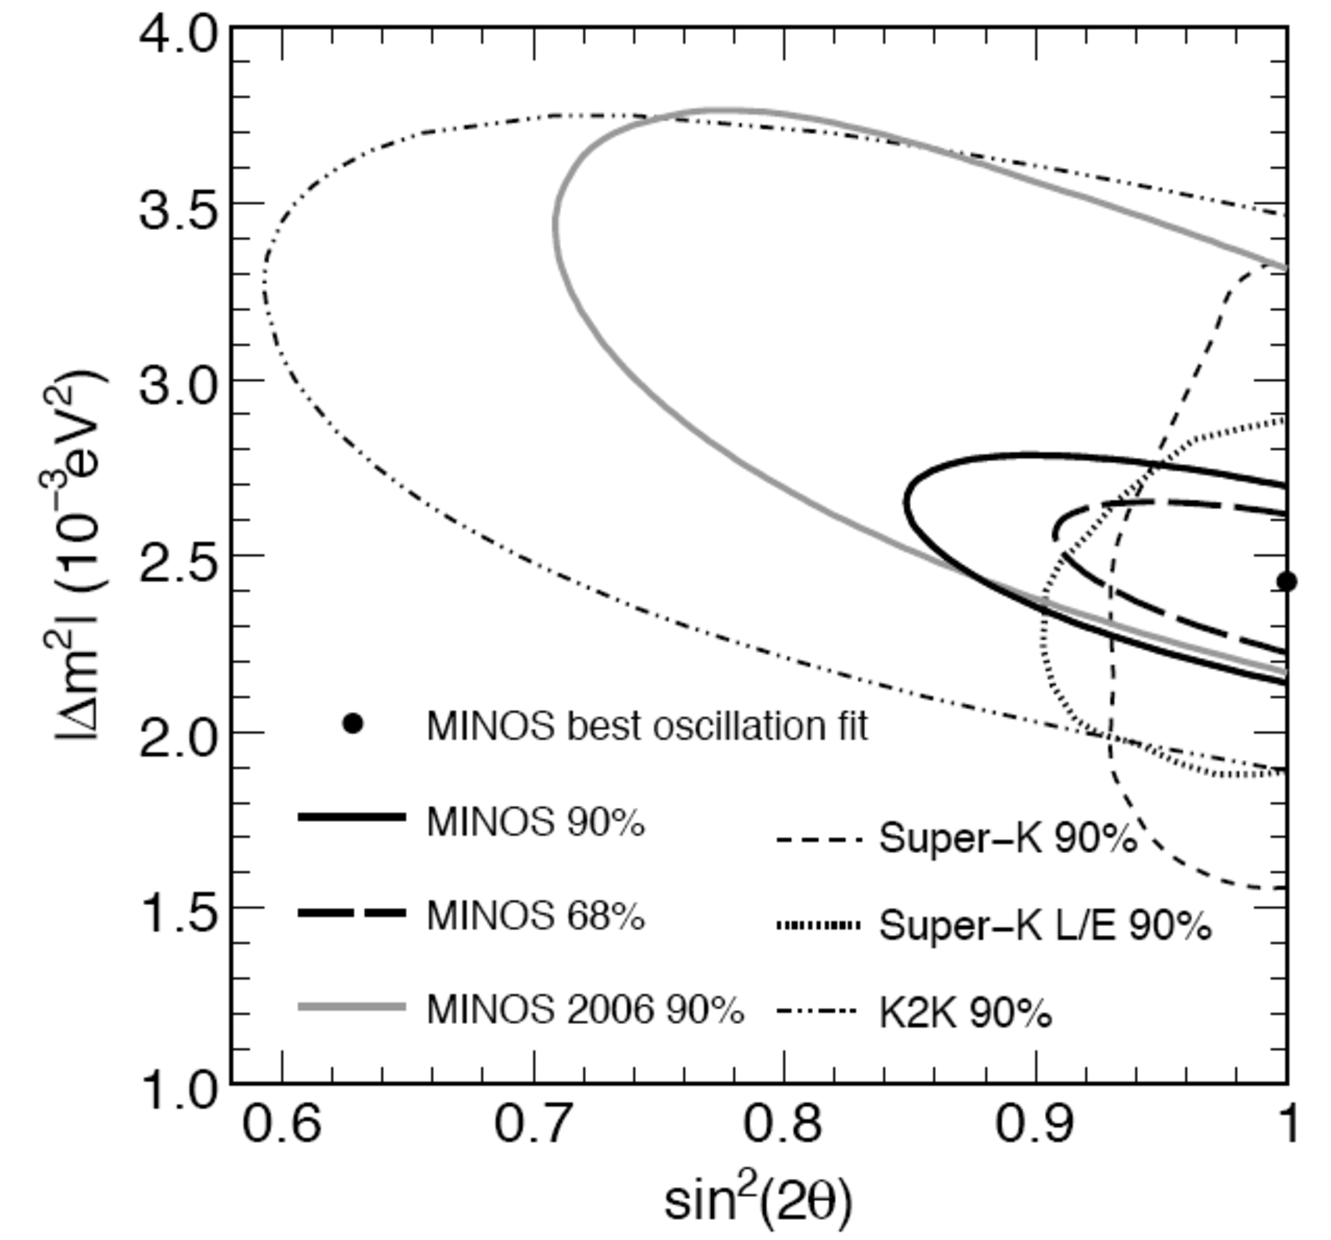
\includegraphics[width=0.6\textwidth]{chapters/neutrinophysics_images/theta_23}
\caption[Allowed region for $\theta_{23}$ and $\Delta m^2_{31}$]{\label{fig:theta_23_confidence}The current knowledge of the values of $\theta_{23}$ and $\Delta m^2_{31}$ as measured by the MINOS, Super-Kamiokande and K2K experiments, with allowed regions at $68\%$ and $90\%$ confidence levels. Figure taken from \citep{PDG2011}.}
\end{figure}

\subsection{Reactor Neutrinos and \texorpdfstring{$\theta_{13}$}{θ₁₃}}
From the PMNS matrix, equation \eqref{eqn:pmns_matrix_combined}, it is clear that the $\Charge\Parity$ violating phase $\delta$ is always associated with a $\sin\theta_{13}$ term. This means that $\Charge\Parity$ violation in the lepton sector requires a non-zero $\theta_{13}$. The T2K~\citep{Abe2011} experiment published indications that $\theta_{13}$ was non-zero in 2011, but the measurement was claimed in 2012 by the Daya Bay reactor neutrino experiment. The Daya Bay collaboration published a result for non-zero $\theta_{13}$ with $5.2\sigma$ significance~\citep{An2012}, quoting a measured value of:
\begin{equation}\label{eqn:reactor_parameters_dyb}
\sin^2 2\theta_{13} = 0.092 \pm 0.016 (\mathrm{stat}) \pm 0.005 (\mathrm{sys})
\end{equation}

Within a month of the Daya Bay result, the RENO reactor neutrino experiment also published a measurement of $\sin^2 2\theta_{13}$~\citep{Ahn2012}:
\begin{equation}\label{eqn:reactor_parameters_reno}
\sin^2 2\theta_{13} = 0.103 \pm 0.013 (\mathrm{stat}) \pm 0.011 (\mathrm{sys})
\end{equation}

Since both the Daya Bay and RENO results are from rate-only analyses, i.e. looking for a deficit of $\bar{\nu}_e$ in the far detector, compared to the flux predicted based on measurements in the near detectors, and in the absence of oscillations, it is reasonably straightforward to combine the two results. The combination process involves averaging the values, weighted by their combined errors (weight $w = 1/\sigma^2$). In order for this to work, the errors should ideally be Gaussian distributed, and uncorrelated. While this is true for the statistical errors, it cannot be trivially assumed for the systematics, which may exhibit some correlation between the two experiments. In the case of the Daya Bay and RENO experiments, however, many of the sources of systematic error are cancelled in the final result due to their use of both near and far detectors. The addition of near detectors allows for flux measurement as well as the cancellation of systematic errors common to both detectors, by taking the ratio of the neutrino flux seen by the near and far detectors. On this basis, it is safe to combine the results of both experiments on the understanding that the remaining systematic errors are uncorrelated between the experiments themselves.

Ideally, such a combination would take the predicted and measured fluxes in each reactor--detector pair (across both experiments), and use a $\chi^2$ minimisation, weighted by the statistical and systematic uncertainties presented for each detector. In the absence of this detailed information, the best one can do is to assume Gaussian, uncorrelated errors, and proceed accordingly. This assumption is somewhat backed up by the parabolic shape of the $\chi^2$ versus $\sin^2 2\theta_{13}$ curves presented by the experiments~\citep{An2012, Ahn2012}.

It turns out that the combined statistical and systematic errors for the two experiments are the same:
\begin{align}
\sigma_{\mathrm{Daya~Bay}} & = \sqrt{0.016^2 + 0.005^2} = 0.017 \\
\sigma_{\mathrm{RENO}} & = \sqrt{0.013^2 + 0.011^2} = 0.017 \nonumber
\end{align}
This simplifies the weighted average to a simple mean:
\begin{equation}
\left<\sin^2 2\theta_{13}\right> = \frac{0.092 + 0.103}{2} = 0.098
\end{equation}
The error on this combined quantity is $\sigma = \sqrt{1 / \sum w}$, which reduces to:
\begin{equation}
\sigma_{\mathrm{Combined}} = \frac{\sigma}{\sqrt{2}} = 0.012
\end{equation}
The combined result is therefore:
\begin{equation}\label{eqn:theta_13_combined}
\left<\sin^2 2\theta_{13}\right> = 0.098 \pm 0.012
\end{equation}

A more thorough combination, bringing in the T2K and MINOS results on $\theta_{13}$, is beyond the scope of this thesis, though such an analysis would allow the production of a confidence region plot showing the parameter space for $\theta_{13}$ and the $\Charge\Parity$ violating phase $\delta$ (the reactor experiments are measuring $\bar{\nu}_e$ disappearance, which is not sensitive to $\delta$; a $\nu_e$ appearance measurement is required).

\begin{figure}
\centering
\rotatebox{-90}{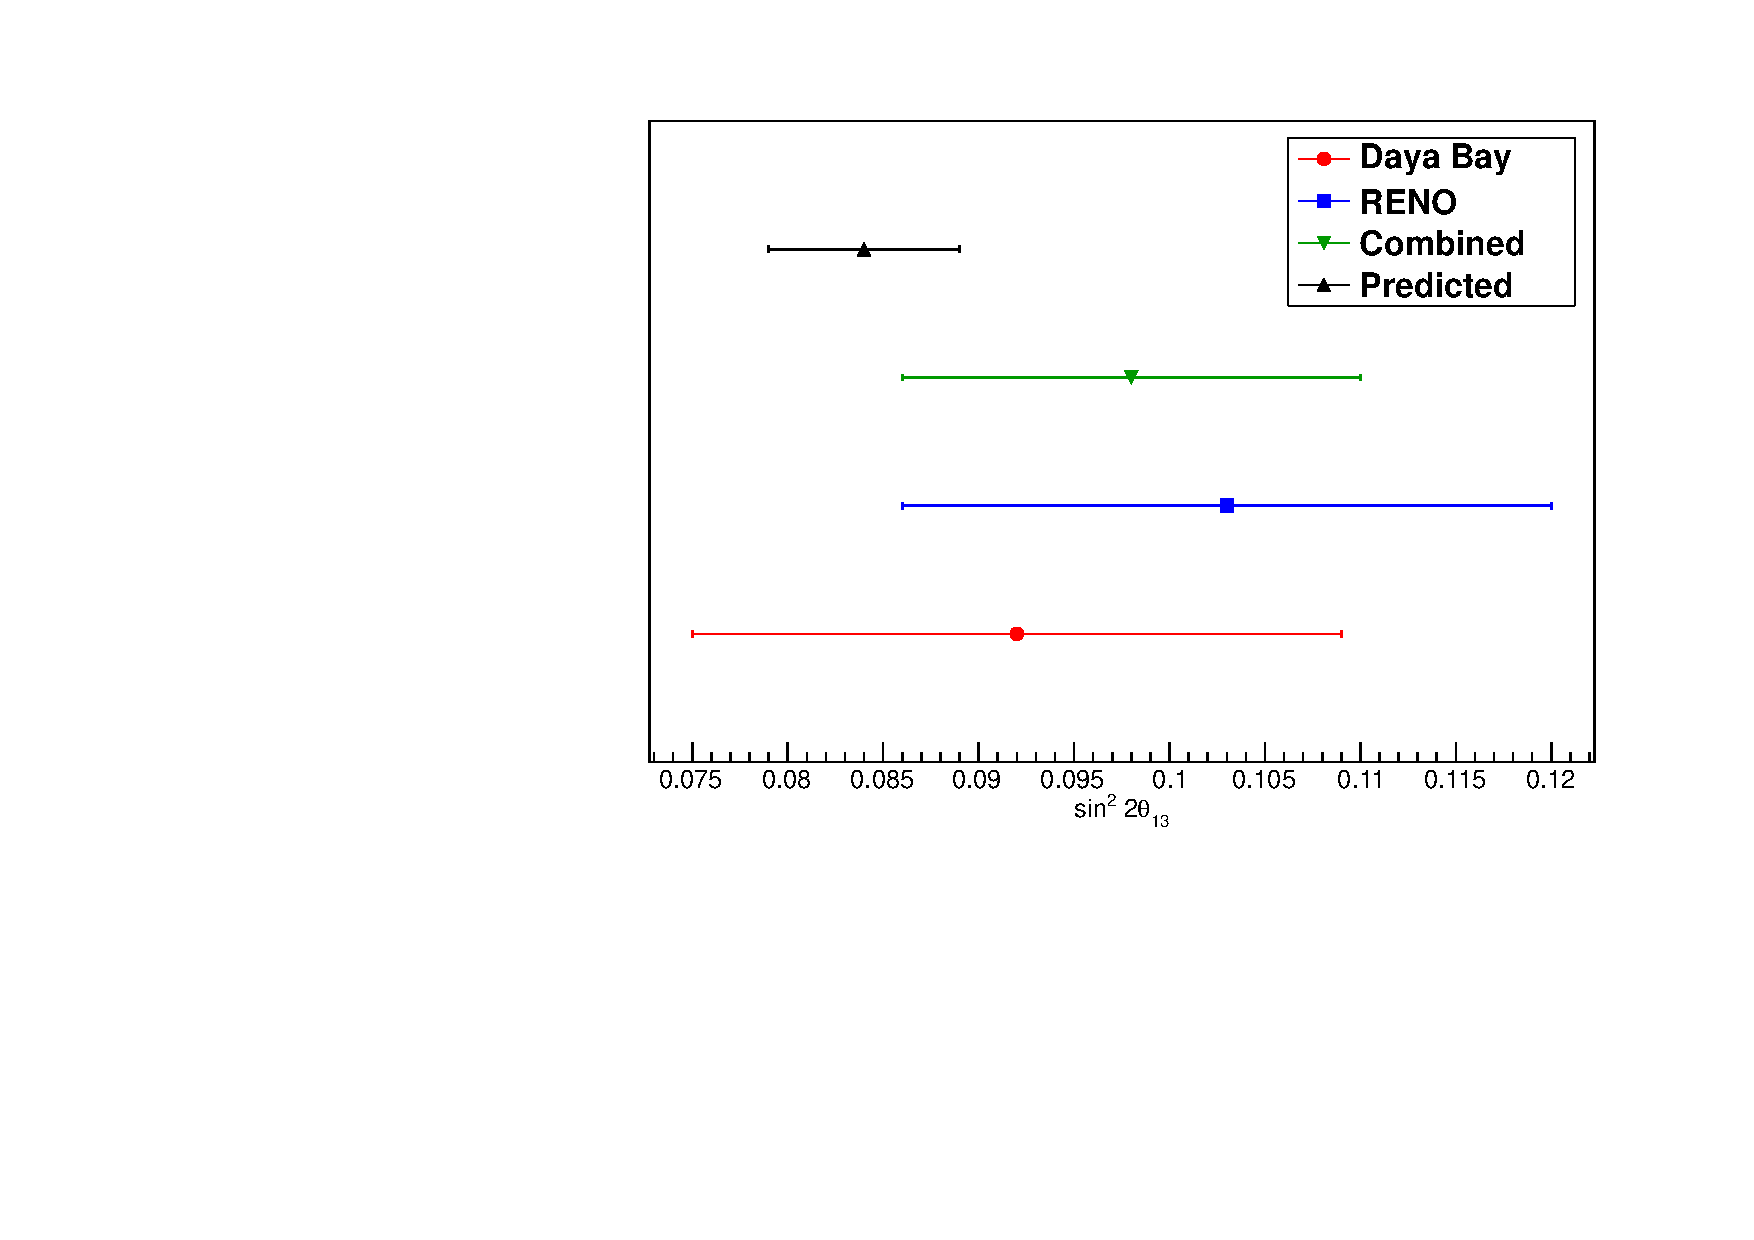
\includegraphics[width=0.6\textwidth]{chapters/neutrinophysics_images/theta_13_results}}
\caption[Comparison of measurements of $\sin^2 2\theta_{13}$]{\label{fig:theta-13_results}Comparison of measurements of $\sin^2 2\theta_{13}$ from the Daya Bay experiment (red), the RENO experiment (blue), a combination of the two results (green) and prediction by Harrison and Scott (black).}
\end{figure}

It is worth noting that in 2004, a prediction compatible with this value of $\sin^2 2\theta_{13}$ was made by Harrison and Scott, by relating $\sin\theta_{13}$ to the two mass-squared differences, $\Delta m^2_{21}$ and $\Delta m^2_{31}$~\citep{Harrison2004}. Their prediction, motivated by the results available at the time, states:
\begin{equation}\label{eqn:theta_13_prediction}
\sin \theta_{13} = \sqrt{\frac{2\Delta m^2_{21}}{3\Delta m^2_{31}}}
\end{equation}

Converting this to a statement about $\sin^2 2\theta_{13}$, and neglecting terms with $\Delta m^4$ (or, equivalently, $\sin^4 \theta$) yields:
\begin{equation}\label{eqn:sin2_2theta_13_prediction}
\sin^2 2\theta_{13} = \frac{8 \Delta m^2_{21}}{3 \Delta m^2_{31}}
\end{equation}
Substituting in the global best-fit values for the two mass splittings, and propagating through the errors, one obtains:
\begin{equation}\label{eqn:prediction_sin2_2theta_13}
\sin^2 2\theta_{13,\,\mathrm{predicted}} = 0.084 \pm 0.005
\end{equation}

The two experimental results, along with the combined result and the predicted value, are shown in figure \ref{fig:theta-13_results}.

\section{Open Questions in Neutrino Physics}
With a non-zero $\theta_{13}$ firmly established, the experimental focus will now shift to the determination of the $\Charge\Parity$ violating phase $\delta$. $\Charge\Parity$ violation in the lepton sector manifests as a difference between the vacuum oscillation probabilities for neutrinos and for antineutrinos, and could form part of an attractive mechanism for generating the observed baryon asymmetry of the universe through processes such as leptogenesis~\citep{Riotto1999}.

Since the sign of the mass splitting $\Delta m^2_{31}$ is not known, there remains a question of \emph{hierarchy}; that is, whether there are two light neutrino mass states and one heavier (the so-called \emph{normal} hierarchy), or two heavy and one light (the \emph{inverted} hierarchy). 

The possible Majorana nature of neutrinos is currently being probed by neutrinoless double-$\beta$ decay experiments, including SuperNEMO~\citep{SuperNEMO} and part of the physics programme for the SNO+ upgrade~\citep{SNO+} to the SNO project.
